\section{Arquitectura de la Aplicación} % (fold)
\label{sec:arquitectura_de_la_aplicacion}
Detrás de la generación de frames se encuentra un sencillo motor gráfico compuesto por una multitud de clases extensibles. En esta sección se examina un poco la arquitectura de este. Sin embargo se hará énfasis detallado en las partes más relevantes al algoritmo de iluminación global.

Una escena en la aplicación está definida por cámaras, luces, materiales, texturas, mallados y un nodo raíz de jerarquía de escena. En la Figura \ref{fig:scene_class_diagram} se muestra un diagrama para las clases que componen una escena.

\begin{figure}[H]
	\centering
	\captionsetup{justification=centering}
	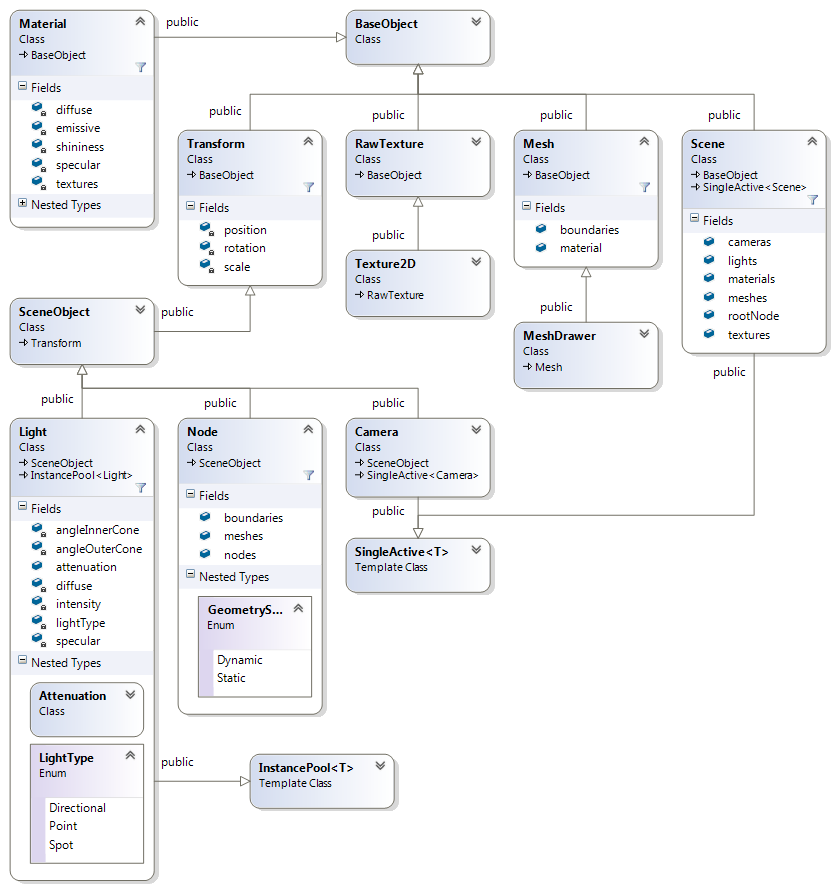
\includegraphics[width=\linewidth]{media/ClassDiagram1.png}
	\caption{Diagrama de clases relevantes para la definición de escenas en el motor gráfico para el renderizado de iluminación global.}
	\label{fig:scene_class_diagram}
\end{figure}

Como se observa en el diagrama cada \emph{Node} o nodo tiene un grupo \emph{meshes} o mallados asociado. Cada una de estas \emph{Mesh} o mallas tiene un material (clase \emph{Material}) asignado, este material puede o no tener uso de texturas. Los nodos en la escena puede definirse como estáticos o dinámicos, esta propiedad es importante para diferenciar entre voxelización estática y dinámica.

Se puede observar también que tanto nodos como mallas tienen un miembro \emph{boundaries} o delimítate, este miembro define una \ac{AABB} utilizada para determinar si estos objetos se encuentran dentro del tronco cuadrado que define el volumen de proyección de la cámara. Esta técnica es llamada \emph{frustum culling}. 

Existen tres tipos de luces en nuestra implementación como ya fue mencionado anteriormente: direccionales, puntuales y focales. Una de las ventajas de realizar el sombreado a través de compute shaders es que podemos colocar muchas luces en escena sin necesidad de crear mapas luz-vista por cada uno de estos.

\begin{figure}[H]
	\centering
	\captionsetup{justification=centering}
	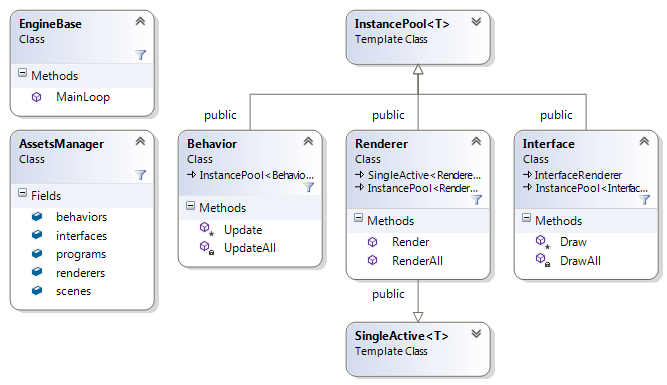
\includegraphics[width=\linewidth]{media/ClassDiagram.png}
	\caption{Diagrama de clases principales con métodos abstractos relacionados con la actualización de cada frame.}
	\label{fig:frame_classes}
\end{figure}

La aplicación utiliza abstracción en el \emph{loop} o ciclo de renderizado. Existen tres clases bases las cuales proveen un método abstracto a implementar por los hijos de estas. Las clases que implementan estos métodos son instanciadas en la clase \emph{AssetsManager}. Por cada instancia de estas clases cada uno de estos métodos es llamado con cada iteración del ciclo de renderizado. Este ciclo incluye la actualización de interfaces, actualización de lógica y actualización de renderizado.

En la Figura \ref{fig:frame_classes} observamos la clase base \emph{Renderer}. En nuestra implementación la voxelización, actualización del mapa de sombras y el cálculo de iluminación global son implementados en clases que heredan de Renderer. La clase \emph{Interface} es la base de todas las interfaces en la aplicación. Mientras que la clase \emph{Behavior} solo es utilizada para lógica de cámara libre flotante en escena.

\begin{figure}[H]
	\centering
	\captionsetup{justification=centering}
	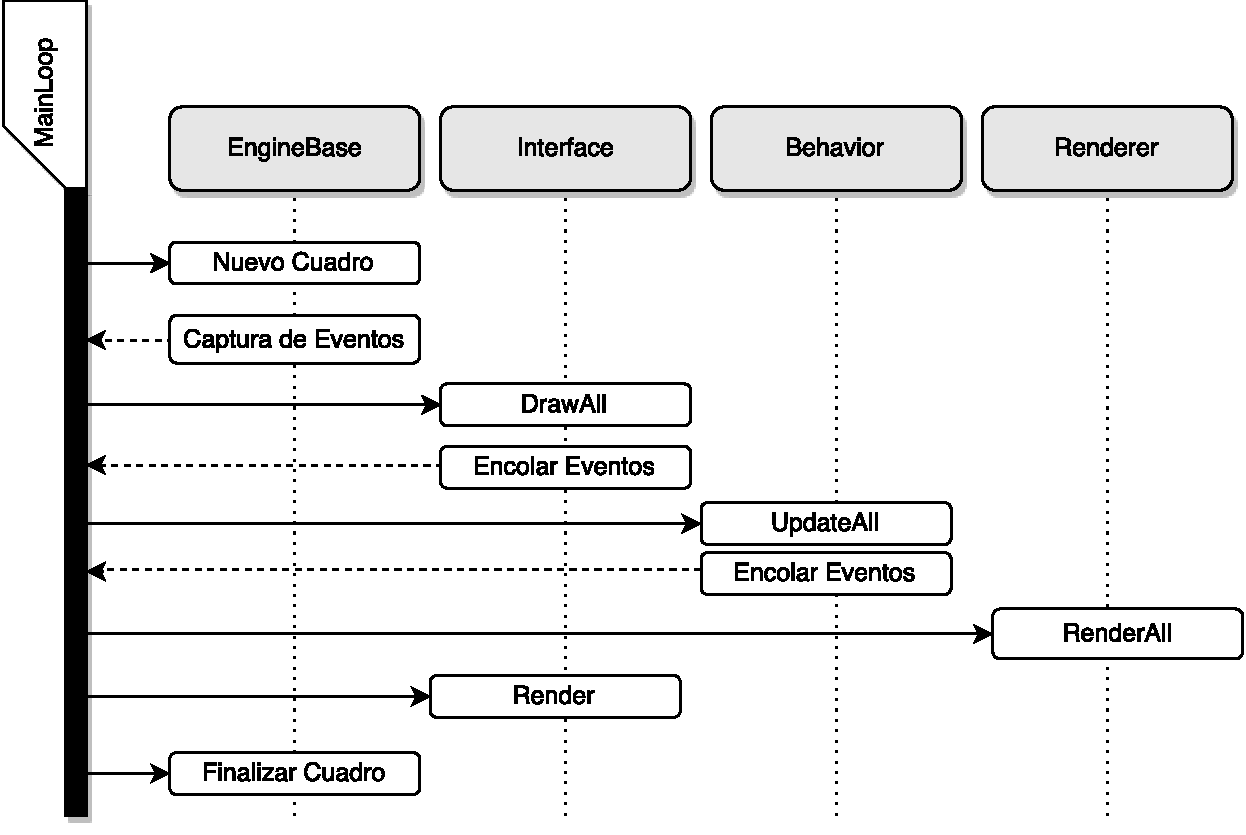
\includegraphics[width=\linewidth]{media/mainloopflow.pdf}
	\caption{Descripción del flujo de ejecución del método \emph{MainLoop} en donde reside el ciclo de renderizado.}
	\label{fig:main_loop}
\end{figure}

Los métodos \emph{Render}, \emph{Draw} y \emph{Update} son abstractos. Mientras que los métodos \emph{RenderAll}, \emph{UpdateAll} y \emph{DrawAll} son métodos estáticos públicos accesibles por la clase \emph{EngineBase}. Estos métodos estáticos invocan a todos las implementaciones de los métodos abstractos por cada clase que hereda de Renderer, Interface o Behavior respectivamente. El método MainLoop en EngineBase por tanto se abstrae de la implementación de estos métodos y simplemente invoca todas las implementaciones por cada nuevo frame. En la Figura \ref{fig:main_loop} se observa el uso de los métodos estáticos para la composición de un frame.
% section arquitectura_de_la_aplicacion (end)
